\documentclass[../problems.tex]{subfiles}

\graphicspath{{../images/}}

% current code highlight settings
\usepackage{listings}
\definecolor{codegreen}{rgb}{0,0.6,0}
\definecolor{codegray}{rgb}{0.5,0.5,0.5}
\definecolor{codepurple}{rgb}{0.58,0,0.82}
\definecolor{backcolour}{rgb}{0.95,0.95,0.92}

\lstdefinestyle{mystyle}{
    backgroundcolor=\color{backcolour},   
    commentstyle=\color{codegreen},
    keywordstyle=\color{magenta},
    numberstyle=\tiny\color{codegray},
    stringstyle=\color{codepurple},
    basicstyle=\ttfamily\footnotesize,
    breakatwhitespace=false,         
    breaklines=true,                 
    captionpos=b,                    
    keepspaces=true,                 
    numbers=left,                    
    numbersep=5pt,                  
    showspaces=false,                
    showstringspaces=false,
    showtabs=false,                  
    tabsize=2
}

\lstset{style=mystyle}

\begin{document}

\section{Newton's Laws of Motion}
\barh

\paragraph{1.1}
Given two vectors $\vect{b} = \vect{\hat x} + \vect{\hat y} $ and $\vect c = \vect{\hat x} + 
\vect{\hat z}$ find $\vect b + \vect c, 5 \vect b + 2 \vect c, \vect b\cdot \vect c$ and $\vect 
b\times \vect c$.
\barh
\begin{equation*}
    \vect{b} + \vect{c} = \vect{\hat x} + \vect{\hat y} + \vect{\hat x} + \vect{\hat z} 
    = 2\vect{\hat x} + \vect{\hat y} + \vect{\hat z}
\end{equation*}
\begin{equation*}
    5 \vect{b} + 2 \vect{c} = 5\vect{\hat x} + 5\vect{\hat y} + 2\vect{\hat x} + 2\vect{\hat z} 
    = 7\vect{\hat x} + 5\vect{\hat y} + 2\vect{\hat z}
\end{equation*}
\begin{equation*}
    \vect{b} \cdot \vect{c} = \vect{\hat x} \cdot \vect{\hat x} + \vect{\hat x} \cdot 
    \vect{\hat z} + \vect{\hat y} \cdot \vect{\hat x} + \vect{\hat y} \cdot \vect{\hat z} 
    = 1 + 0 + 0 + 0 = 1
\end{equation*}
\begin{equation*} %using the determinant
    \vect{b} \times \vect{c} = \det \begin{bmatrix}
        \vect{\hat x} & \vect{\hat y} & \vect{\hat z} \\
        1 & 1 & 0 \\
        1 & 0 & 1
    \end{bmatrix}
    = \vect{\hat x} - \vect{\hat y} - \vect{\hat z}
\end{equation*}

\paragraph{1.2}
Given Vectors $\vect{b}=(1,2,3) ,\ \vect{c} = (3,2,1)$ compute 1.1
\barh
\begin{equation*}
    \vect{b} + \vect{c} = (4,4,4)
\end{equation*}
\begin{equation*}
    5 \vect{b} + 2 \vect{c} = (5,10,15) + (6,4,2) = (11,14,17)
\end{equation*}
\begin{equation*}
    \vect{b} \cdot \vect{c} = 1(3) + 2(2) + 3(1) = 10
\end{equation*}
\begin{equation*}
    \vect{b} \times \vect{c} = \det \begin{bmatrix}
        \vect{\hat x} & \vect{\hat y} & \vect{\hat z} \\
        1 & 2 & 3 \\
        3 & 2 & 1
    \end{bmatrix}
    = -4\vect{\hat x} + 8\vect{\hat y} - 4\vect{\hat z}
\end{equation*}

\paragraph{1.3}
Pythagorean Theorem for three dimensions
\barh

First find the magntitude of the vector $\vect{a} = x + y$ made up of the x and y components 
\begin{equation*}
    |\vect{a}| = \sqrt{x^2 + y^2}
\end{equation*}

Then the magnitude of the vector $\vect{r} = a + z$ made up of the x, y, and z components
\begin{align*}
    |\vect{r}| = \sqrt{x^2 + y^2 + z^2} \\
    r^2 = x^2 + y^2 + z^2
\end{align*}

\paragraph{1.4}
Find $\angle$ between vectors $\vect{b}= (1,2,4) ,\  \vect{c} = (4,2,1)$ using dot product
\barh
\begin{gather*}
    \vect{b}\cdot \vect{c} = 1(4) + 2(2) + 4(1) = 12 \\
    |\vect{b}| = \sqrt{1^2 + 2^2 + 4^2} = \sqrt{21} \\
    |\vect{c}| = \sqrt{4^2 + 2^2 + 1^2} = \sqrt{21} \\
    \cos \theta = \frac{\vect{b}\cdot \vect{c}}{|\vect{b}||\vect{c}|} = \frac{12}{21} \\
    \theta = \cos^{-1} \frac{12}{21} = 55^\circ
\end{gather*}

\paragraph{1.5}
Angle between cube body diagonal and face diagonal
\barh

Face diagonal vector $\vect{P} = (1,1,0)$ and Body Diagonal $\vect{Q} = (1,1,1)$
\begin{gather*}
    \vect{P} \cdot \vect{Q} = 1 + 1 + 0 = 2 \\
    |\vect{P}| = \sqrt{2} \qquad |\vect{Q}| = \sqrt{3} \\
    \cos \theta = \frac{2}{\sqrt{6}} \\
    \theta = 35^\circ
\end{gather*}

\paragraph{1.6}
Find scalar $s$ for orthogonal vectors $\vect{B} =  \vect{\hat x} + s \vect{\hat y} , \  \vect{C} 
= \vect{\hat x} - s\vect{\hat y}$
\barh

The dot product of orthgonal vectors is zero: 
\begin{gather*}
    \vect{B} \cdot \vect{C} = 0 \\
    (1, s) \cdot (1, -s) = 1 - s^2 = 0 \\
    s^2 = 1 \\
    s = \pm 1
\end{gather*}

\paragraph{1.7}
Prove the 2 definitions of scalar product are equal
\barh

Treat vector $\vect{r}$ stricly in the x axis: $\vect{r} = (x,0,0)$ and $\vect{s} 
= (s_x, s_y, s_z)$:
\begin{figure}[ht]
    \centering
    \def\svgwidth{170px}
    \input{images/fig1_7.pdf_tex}
    \caption{}
\end{figure}

the x component of the vector $s_x$ is equivalent to $s \cos{\theta}$... 

\begin{align*}
    \vect{r}\cdot \vect{s} &= |\vect{r}| |\vect{s}| \cos{\theta} & &=\sum_{i=1}^3 r_i s_i\\
    &= x s \cos{\theta}  &  &= x s_x\\
    &= x s_x 
\end{align*}

\paragraph{1.8}
Prove dot product is distributive and differentiable
\barh

\begin{align*}
    (\vect{a}+\vect{b})\cdot \vect{c} &= \sum_{i=1}^3 (a_i + b_i) c_i \\
    &= \sum_{i=1}^3 a_i c_i + \sum_{i=1}^3 b_i c_i \\
    &= \vect{a}\cdot \vect{c} + \vect{b}\cdot \vect{c}
\end{align*}
% end with vectors a dot b = a dot db/dt + da/dt dot b
\begin{align*}
    \frac{d}{dt} (\vect{a}\cdot \vect{b}) &= \frac{d}{dt} \sum_{i=1}^3 a_i b_i \\
    &= \sum_{i=1}^3 \frac{d}{dt} a_i b_i \\
    &= \sum_{i=1}^3 \frac{da_i}{dt} b_i + \sum_{i=1}^3 a_i \frac{db_i}{dt} \\
    &= \frac{d\vect{a}}{dt} \cdot \vect{b} + \vect{a} \cdot \frac{d\vect{b}}{dt}
\end{align*}

\paragraph{1.9}
Show law of cosines from the identity $(\vect{a} + \vect{b})^2 = a^2 + b^2 + 2 \vect{a} \cdot 
\vect{b}$
\barh

\begin{figure}[ht]
    \centering
    \includegraphics{fig1_9.png}
    \caption{Law of Cosine: $c^2 = a^2 + b^2 - 2ab\cos{\theta}$}
\end{figure}

Using the identity $\cos{\phi} = \cos{(\pi - \phi)} = - \cos{\theta}$
\begin{align*}
    \vect{c}^2 &= (\vect{a} + \vect{b})^2 \\
    &= a^2 + b^2 + 2 \vect{a} \cdot \vect{b} \\
    &= a^2 + b^2 + 2 |\vect{a}||\vect{b}| \cos{\phi} \\
    &= a^2 + b^2 - 2 ab \cos{\theta} \\
    &= a^2 + b^2 - 2ab\cos{\theta}
\end{align*}

\paragraph{1.11}
Describe the orbit of a particle with the position function $r(t) = \vect{\hat x} b \cos{\omega t} 
+ \vect{\hat y} c \sin{\omega t}$
\barh

This is a parametric representation of an ellipse using trigonometric functions 
$x = b \cos{\omega t}$, $y = c \sin{\omega t}$
equivalent to the standard ellipse equation:
\begin{equation*}
    \frac{x^2}{b^2} + \frac{y^2}{c^2} = 1
\end{equation*}

The particle is moving counter-clockwise in the x-y plane with semi-major(longer) axis and 
semi-minor(short) axis $c$ and $b$.

\begin{figure}[ht]
    \centering
    \includegraphics[scale=0.8]{fig1_11.png}
    \caption{Ellipse with semi-major axis $b$ and semi-minor axis $c$}
\end{figure}

\newpage
\paragraph{1.13}
For a fixed unit vector $\vect{u}$ show the any vector $\vect{b}$ satisfies 
$b^2 = (\vect{b}\cdot \vect{u})^2 + (\vect{b}\times \vect{u})^2$
\barh

The magnitude of a unit vector is 1
\begin{align*}
    b^2 &= (b \sin{\theta})^2 + (b \cos{\theta})^2 \\
\end{align*}

This is equivalent to the Pythagorean Theorem.
\begin{figure}[ht]
    \centering
    \includegraphics[scale=0.9]{fig1_13.png}
    \caption{}
\end{figure}

\paragraph{1.15}
Show $\vect{r} \times \vect{s}$ is perpendicular to both $\vect{r}$ and $\vect{s}$ with magnitude 
$rs \sin{\theta}$ given by the right-hand rule
\barh

Choosing $\vect{r} = (r, 0, 0) , \vect{s} = (s_x, s_y, 0)$ where $s_y = s \sin{\theta}$
\begin{align*}
    \vect{r} \times \vect{s} &= \det \begin{bmatrix}
        \vect{\hat x} & \vect{\hat y} & \vect{\hat z} \\
        r_x & 0 & 0 \\
        s_x & s_y & 0
    \end{bmatrix} \\
    &= -r_x s_y \vect{\hat z} \\
    &= rs \sin{\theta} \vect{\hat z}
\end{align*}

    The result is a vector stricly in the z direction, orthogonal to the x-y plane. 

\paragraph{1.17}
(a) Prove the vector product is distributive as in: $\vect{r} \times (\vect{u} + \vect{v}) 
= \vect{r} \times \vect{u} + \vect{r} \times \vect{v}$ (b) and differentiable by product rule
\begin{equation*}
    \frac{d}{dt} (\vect{r} \times \vect{s}) = \frac{d\vect{r}}{dt} \times \vect{s} + \vect{r} 
    \times \frac{d\vect{s}}{dt}
\end{equation*}
\barh

(a) The components of the vector cross product $\vect{p} = \vect{r} \times \vect{s}$
\begin{equation} \tag{1.9} \label{eq1.9}
\begin{split}
    p_x &= r_y s_z - r_z s_y \\
    p_y &= r_z s_x - r_x s_z \\
    p_z &= r_x s_y - r_y s_x
\end{split}
\end{equation}

Starting with the x componenet of the the resultant vector
\begin{align*}
    \vect{r} \times (\vect{u} + \vect{v}) &= \det \begin{bmatrix}
        \vect{\hat x} & \vect{\hat y} & \vect{\hat z} \\
        r_x & r_y & r_z \\
        u_x + v_x & u_y + v_y & u_z + v_z
    \end{bmatrix} \\
    &= r_y(u_z + v_z) - r_z(u_y + v_y) \\
    &= (r_y u_z - r_z u_y) + (r_y v_z - r_z v_y) \\
    &= (r \times u)_x + (r \times v)_x 
\end{align*}

The same can be done for the y and z components to show that the product is distributive.

\newpage
(b) Using \eqref{eq1.9} starting with just the x component again
\begin{align*}
    \frac{d}{dt} [(\vect{r} \times \vect{s})_x] &= \frac{d}{dt} [r_y s_z - r_z s_y] \\
    &= \frac{dr_y}{dt} s_z + r_y \frac{ds_z}{dt} - \frac{dr_z}{dt} s_y - r_z \frac{ds_y}{dt} 
    = \left(\frac{dr_y}{dt}s_z - \frac{dr_z}{dt} s_y\right) 
    + \left(  r_y \frac{ds_z}{dt} + r_z \frac{ds_y}{dt} \right) \\
    &= \left[ \frac{d\vect{r}}{dt} \times \vect{s} 
    + \vect{r} \times \frac{d\vect{s}}{dt} \right]_x
\end{align*}

id. can the done in the y and z components to prove the product rule.

\paragraph{1.19}
If $\vect{r}$, $\vect{v}$, and $\vect{a}$ are the position, velocity, and acceleration vectors of a 
particle, prove that
\begin{equation*}
    \frac{d}{dt} [\vect{a} \cdot (\vect{v} \times \vect{r})] = \vect{\dot a} \cdot (\vect{v} 
    \times \vect{r})
\end{equation*}
\barh

Using the product rule for the dot product
\begin{align*}
    \frac{d}{dt} [\vect{a} \cdot (\vect{v} \times \vect{r})] 
    &= \frac{d\vect{a}}{dt} \cdot (\vect{v} \times \vect{r}) 
    + \vect{a} \cdot \frac{d}{dt} (\vect{v} \times \vect{r}) \\
    &= \vect{\dot a} \cdot (\vect{v} \times \vect{r}) 
    + \vect{a} \cdot \frac{d\vect{v}}{dt} \times \vect{r} 
    + \vect{a} \cdot \vect{v} \times \frac{d\vect{r}}{dt} \\
    &= \vect{\dot a} \cdot (\vect{v} \times \vect{r}) 
    + \vect{a} \cdot \vect{a} \times \vect{r} + \vect{a} \cdot \vect{v} \times \vect{v} \\
    &= \vect{\dot a} \cdot (\vect{v} \times \vect{r})
\end{align*}

The cross product of a vector with itself is zero. $\vect{a} \times \vect{a} = 0$ and the dot 
product of orthogonal vectors is zero.

\paragraph{1.21}
Show the volume of a parallelepiped defined by vectors $\vect{a}$, $\vect{b}$, and $\vect{c}$ is 
$V = |\vect{a} \cdot (\vect{b} \times \vect{c})|$
\barh

In geometry, the cross product refers to the positive area of a parallelgram(directed area 
product) which is the base area of the parallelepiped.
\begin{equation*}
    \vect{b} \times \vect{c} = bc \sin{\theta} = \text{base area}
\end{equation*}

The dot product equates to the volume of the parallelepiped with height $\vect{a}\cos{\phi}$... 
\href{https://en.wikipedia.org/wiki/Triple_product}{scalar triple product}

\paragraph{1.23}
The unknown vector $\vect{b}$ satisfies $\vect{b} \cdot \vect{v} = \lambda$ and $\vect{b} \times 
\vect{v} = \vect{c}$. Find $\vect{v}$ in terms of $\lambda$, $\vect{b}$, and $\vect{c}$.
\barh

\begin{figure} [ht]
    \centering 
    \includegraphics[scale=0.9]{fig1_23.png}
    \caption{Visual example of vector $\vect{b}$ and $\vect{v}$ with vector $\vect{c}$ pointing 
    into the page}
    \label{fig1.5}
\end{figure}

$\vect{v}$ can be expressed as a linear combination of 2 orthogonal vectors

\begin{equation*}
    \vect{v} = \alpha \vect{b} + \beta \vect{b} \times \vect{c}
\end{equation*}

\newpage
Taking the dot product to solve for $\alpha$
\begin{align*}
    \vect{b} \cdot \vect{v} &= \vect{b} \cdot (\alpha \vect{b} 
    + \beta \vect{b} \times \vect{c}) \\
    &= \alpha \vect{b} \cdot \vect{b} + \beta \vect{b} \cdot (\vect{b} \times \vect{c}) \\
    \lambda &= \alpha b^2 \\
    \alpha &= \frac{\lambda}{b^2}
\end{align*}

\ref{fig1.5} shows that $\vect{b} \times \vect{c}$ is orthogonal to $\vect{b}$ so the dot 
product is zero. Solving for $\beta$
\begin{align*}
    \vect{b} \times \vect{v} &= \vect{b} \times (\alpha \vect{b} 
    + \beta \vect{b} \times \vect{c}) \\
    &= \alpha \vect{b} \times \vect{b} + \beta \vect{b} \times (\vect{b} \times \vect{c}) \\
    &= \beta \vect{b} \times (\vect{b} \times \vect{c}) \\
    &= \beta \vect{b} (b^2 c) \\
    &= \beta (-b^2 c) 
\end{align*}

The direction of the resultant triple product is in the negative direction of $\vect{c}$ so 
$\beta = -\frac{1}{b^2}$

\begin{equation*}
    \vect{v} = \frac{\lambda}{b^2} \vect{b} - \frac{1}{b^2} \vect{b} \times \vect{c}
\end{equation*}

\paragraph{1.25}
Find the general solution for the first-order differential equation $df/dt = -3f$
\barh
    
\begin{align*}
    \frac{df}{dt} &= -3f \\
    \int \frac{1}{f} df &= \int -3 dt \\
    \ln{f} &= -3t + C \\
    f &= e^{-3t + C} \\
    f &= Ae^{-3t}
\end{align*}

\paragraph{1.29} 
Go over the steps from (1.25) to (1.29) for the conservation of momentum for $N=4$ particles
\barh

\begin{equation} \tag{1.25} \label{eq1.25}
    (\text{net force on particle}) = \vect{F}_\alpha =
    \sum_{\beta \neq \alpha} \vect{F}_{\alpha \beta} + \vect{F}_{\alpha}^\text{ext}
\end{equation}

Where $\vect{F}_{\alpha \beta}$ denotes the force on particle $\alpha$ due to particle $\beta$
\begin{equation} \tag{1.26} \label{eq1.26}
    \dot{\vect{p}}_\alpha = \sum_{\beta \neq \alpha} \vect{F}_{\alpha \beta} 
    + \vect{F}_{\alpha}^\text{ext}
\end{equation}

This is in accordance to Newton's second law, same as the rate of change of momentum 
$\vect{p}_\alpha$. For the total momentum of the particle $\vect{P}$
\begin{equation} \tag{1.27} \label{eq1.27}
    \dot{\vect{P}} = \sum_{\alpha}^N \dot{\vect{p}}_\alpha =
    \sum_{\alpha}^N \sum_{\beta \neq \alpha} \vect{F}_{\alpha \beta} + 
    \sum_{\alpha}^N \vect{F}_{\alpha}^\text{ext}
\end{equation}

Reorganizing double sum
\begin{equation} \tag{1.28} \label{eq1.28}
    \sum_{\alpha}^N \sum_{\beta \neq \alpha} \vect{F}_{\alpha \beta} 
    = \sum_{\alpha}^N \sum_{\beta > \alpha} (\vect{F}_{\alpha \beta} + \vect{F}_{\beta \alpha}) 
\end{equation}
    
Since the terms in double sum \eqref{eq1.28} is zero by Newton's third law
\begin{equation} \tag{1.29} \label{eq1.29}
    \dot{\vect{P}} = \sum_{\alpha}^N \vect{F}_{\alpha}^\text{ext} \equiv \vect{F}^\text{ext}
\end{equation}

\newpage
\eqref{eq1.25} and \eqref{eq1.26} for $N=4$ particles
\begin{align*}
    \dot{\vect{p}}_1 &= \vect{F}_{12} + \vect{F}_{13} + \vect{F}_{14} + \vect{F}_{1}^\text{ext} \\
    \dot{\vect{p}}_2 &= \vect{F}_{21} + \vect{F}_{23} + \vect{F}_{24} + \vect{F}_{2}^\text{ext} \\
    \dot{\vect{p}}_3 &= \vect{F}_{31} + \vect{F}_{32} + \vect{F}_{34} + \vect{F}_{3}^\text{ext} \\
\end{align*}

Summation of momentum \eqref{eq1.27} $\dot{\vect{P}} = \dot{\vect{p}}_1 + \dot{\vect{p}}_2 
+ \dot{\vect{p}}_3 + \dot{\vect{p}}_4$
\begin{align*}
    \dot{\vect{P}} = (\vect{F}_{12} + \vect{F}_{13} + \vect{F}_{14} + \vect{F}_{1}^\text{ext}) 
    + (\vect{F}_{21} + \vect{F}_{23} + \vect{F}_{24} + \vect{F}_{2}^\text{ext}) \\
    + (\vect{F}_{31} + \vect{F}_{32} + \vect{F}_{34} + \vect{F}_{3}^\text{ext}) + (\vect{F}_{41} 
    + \vect{F}_{42} + \vect{F}_{43} + \vect{F}_{4}^\text{ext})
\end{align*}

Reorganizing the double sum like \eqref{eq1.28}
\begin{align*}
    \dot{\vect{P}} = (\vect{F}_{12} + \vect{F}_{21}) + (\vect{F}_{13} + \vect{F}_{31}) 
    + (\vect{F}_{14} + \vect{F}_{41}) + (\vect{F}_{23} + \vect{F}_{32}) \\
    + (\vect{F}_{24} + \vect{F}_{42}) + (\vect{F}_{34} + \vect{F}_{43}) + (\vect{F}_{1}^\text{ext} 
    + \vect{F}_{2}^\text{ext} + \vect{F}_{3}^\text{ext} + \vect{F}_{4}^\text{ext})
\end{align*}

By Newton's third law, the opposing forces cancel out
\begin{equation*}
    \dot{\vect{P}} = \vect{F}_{1}^\text{ext} + \vect{F}_{2}^\text{ext} + \vect{F}_{3}^\text{ext} 
    + \vect{F}_{4}^\text{ext} \equiv \vect{F}^\text{ext}
\end{equation*}

\paragraph{1.31}
The law of conservation of momentum says that if there are no external forces on this pair of 
particles, then their total momentum must be constant. Use this to prove that 
$\vect{F}_{12} = -\vect{F}_{21}$.
\barh

\begin{equation*}
    \dot{\vect{P}} = \vect{F}_{1}^\text{ext} + \vect{F}_{2}^\text{ext} \equiv \vect{F}^\text{ext}
\end{equation*}

For a two particle system

\begin{equation*}
    \dot{\vect{P}} = \vect{F}_{12} + \vect{F}_{21} + \vect{F}^{\text{ext}}
\end{equation*}

If there are no external forces, then $\vect{F}^\text{ext} = 0$ and for total momentum to be 
constant, $\dot{\vect{P}} = 0$. Therefore the interparticle forces obey the third law i.e.
$\vect{F}_{12} = -\vect{F}_{21}$

\paragraph{1.33}
Prove the magnetic forces, $\vect{F}_{12}$ and $\vect{F}_{21}$, between two steady current loops 
obey Newton's 3rd law
\barh

\textit{Hints}: for currents $I_1$ and $I_2$, and points $r_1$ and $r_2$. According to Bio-Savart 
Law, the force on the segment $d\vect{r}_1$ due to $d\vect{r}_2$ of loop 2 is
\begin{equation*}
    \frac{\mu_0}{4\pi} \frac{I_1 I_2}{s^2} d\vect{r}_1 \times (d\vect{r}_2 \times \vect{\hat s})
\end{equation*}
where $\vect{s} = \vect{r_1} - \vect{r_2}$. The force $\vect{F_{12}}$ is found integrating over both
loops. The unit vector is equivalent to
\begin{equation*}
    \hat{\vect{s}} = \frac{\vect{s}}{s} = \frac{\vect{r_1} - \vect{r_2}}{|\vect{r_1} - \vect{r_2}|}
\end{equation*}
and the \emph{BAC - CAB} identity for the triple product
\begin{equation*}
    \vect{a} \times (\vect{b} \times \vect{c}) = \vect{b}(\vect{a} \cdot \vect{c}) 
    - \vect{c}(\vect{a} \cdot \vect{b})
\end{equation*}

Integrating over both loops the force on loop 1 due to loop 2
\begin{align*}
    \vect{F}_{12} &= \oint \oint \frac{\mu_0}{4\pi} \frac{I_1 I_2}{s^2} d\vect{r}_1 
    \times (d\vect{r}_2 \times \vect{\hat s})
\end{align*}

Using the \emph{BAC - CAB} identity
\begin{align*}
    \vect{F}_{12} &= \frac{\mu_0}{4\pi} I_1 I_2 \left[
        \oint \oint \frac{d\vect{r}_2 (d\vect{r}_1 \cdot \hat{\vect{s}})}{s^2} 
        - \oint \oint \frac{\hat{\vect{s}} (d\vect{r}_1 \cdot d\vect{r}_2)}{s^2} \right] \\
\end{align*}

\newpage
In the first term, the dot product $d\vect{r_1} \cdot \hat{\vect{s}}$ is projection of in the 
direction of $\vect{s}$ and the integral of the closed current loop is zero
\begin{equation*}
    \oint_{C_2} \oint_{C_1} \frac{d\vect{r}_2 (d\vect{r}_1 \cdot \hat{\vect{s}})}{s^3} 
    = \oint_{C_2} d\vect{r_2} \oint_{C_1} \frac{ds}{s^2} = 0
\end{equation*}

We end up with the force on loop 1 due to loop 2 as 
\begin{equation*}
    \vect{F}_{12} = -\frac{\mu_0}{4\pi} I_1 I_2 \oint_{C_2} \oint_{C_1} \frac{\hat{\vect{s}} 
    (d\vect{r}_1 \cdot d\vect{r}_2)}{s^2} = -\vect{F}_{21}
\end{equation*}

\paragraph{1.35}
A golf ball is hit from ground level due east at a velocity $v_0$ at an angle $\theta$ above the 
horizontal. Neglecting air resistance use Newton's Second Law to find position as a function of 
time, the time for the ball to hit the ground, and the range of the ball. x measures east, y north, 
and z vertically up.
\barh

Newton's second law states $\vect{F} = m\ddot{\vect{r}}$ where $\ddot{\vect{r}} = \vect{g} 
= -g\vect{\hat z}$ is the gravitational force. We can find the position of the ball by integrating 
twice with respect to time
\begin{align*}
    \ddot{x} &= 0 &              \ddot{y} &= 0                & \ddot{z} &= -g\\ 
    \dot{x} &= 0 & \dot{y} &= 0 &            \dot{z} &= -gt + v_0 \sin{\theta} \\
    x(t) &= 0      & y(t) &= 0 &       z(t) &= -\frac{1}{2}gt^2 + v_0 t\sin{\theta} 
\end{align*}

The time for the ball to hit the ground is when $z(t) = 0$
\begin{align*}
    -\frac{1}{2}gt^2 + v_0 t\sin{\theta} &= 0 \\
    t &= \frac{2v_0 \sin{\theta}}{g}
\end{align*}

To get the range of the ball we subsitute $t$ from above into $x(t)$
\begin{align*}
    x(t) &= v_0 \cos{\theta} \frac{2v_0 \sin{\theta}}{g} \\
    x(t) &= \frac{2v_0^2 \sin{\theta} \cos{\theta}}{g} \\
    x(t) &= \frac{v_0^2 \sin{2\theta}}{g}
\end{align*}

\paragraph{1.37}
A student kicks a frictionless puck with initial speed $v_0$, so that it slides straight up a plane 
that is inclined at an angle $\theta$ above the horizontal (a) Write down Newton’s second law for 
the puck and solve to give its position as a function of time (b) How long will the puck take to 
return to its starting point?
\barh

(a) Having the x-axis on the plane parallel to the incline we get the force equation
\begin{equation*}
    F_x = m\ddot{x} = -mg\sin{\theta}
\end{equation*}

Solving for the position of the puck by integrating twice with respect to time and using the initial 
conditions $x(0) = 0$ and $\dot{x}(0) = v_0$
\begin{align*}
    \ddot{x} &= -g\sin{\theta} \\
    \dot{x} &= g\cos{\theta} t + v_0 \\
    x(t) &= -\frac{1}{2}g\sin{\theta} t^2 + v_0 t
\end{align*}

(b) Solving for when the puck returns to its starting point $x(t) = 0$
\begin{align*}
    -\frac{1}{2}g\sin{\theta} t^2 + v_0 t &= 0 \\
    t &= \frac{2v_0}{g\sin{\theta}}
\end{align*}

\paragraph{1.39}
Show the ball lands a distance $R =2 v_o^2 \sin{\theta} \cos{\left(\theta + \phi\right)}/
\left( g \cos^2{\phi} \right)$ and $R_{max} = v_o^2/[g(1+ \sin{\phi})]$
\barh
Using $\theta$ as the angle above the incline and $\phi$ as the angle of the incline plane
the components of the inital velocity are
\begin{align*}
    v_{ox} = v_0 \cos{\theta} \quad v_{oy} = v_0 \sin{\theta} \quad v_{oz} = 0
\end{align*}
Newton's second law
\begin{align*}
    F_x &= -m g \sin{\phi} & F_y &= -m g \cos{\phi} & F_z &= 0 \\
    \ddot{x} &= -g \sin{\phi} & \ddot{y} &= -g \cos{\phi} & \ddot{z} &= 0 \\
    \dot{x} &= -g \sin{\phi} t + v_{ox} & \dot{y} &= -g \cos{\phi} t + v_{oy} & \dot{z} & = 0 \\
    x(t) &= -\frac{1}{2} g \sin{\phi} t^2 + v_{ox} t & y(t) &= -\frac{1}{2} g \cos{\phi} t^2 
    + v_{oy} t & z(t) &= 0
\end{align*}

The range of the ball is when $y(t) = 0$ as it lands on the incline plane
\begin{align*}
    0 = -\frac{1}{2} g \cos{\phi} t^2 + v_{oy} t \\
    t = \frac{2 v_{oy}}{g \cos{\phi}}
\end{align*}

Substituting $t$ into $x(t)$ and using the identity $\cos{\left(\theta \pm \phi\right)} 
= \cos{\theta} \cos{\phi} \mp \sin{\theta} \sin{\phi}$ simplifies the range...
\begin{align*}
    x (t) &= -\frac{1}{2} g \sin{\phi} \left( \frac{2 v_{oy}}{g \cos{\phi}} \right)^2 + v_{ox} 
    \left( \frac{2 v_{oy}}{g \cos{\phi}} \right) \\
    R &= \frac{-2 v_o^2}{g\cos^2{\phi}} \sin^2{\theta} \sin{\phi} 
    + \frac{2 v_o^2}{g\cos{\phi}} \sin{\theta} \cos{\theta} \\
    &= \frac{2v_o^2 \sin{\theta}}{g \cos^2{\phi}} \left( -\sin{\theta} \sin{\phi} 
    + \cos{\theta} \cos{\phi} \right) \\
    R &= \frac{2v_o^2 \sin{\theta}}{g \cos^2{\phi}} \cos{\left(\theta + \phi\right)}
\end{align*}

Set identity $\sin{\alpha}\cos{\beta}=1/2[\sin{(\alpha+\beta)}+\sin{(\alpha-\beta)}]$
\begin{align*}
    \frac{dR}{d\theta} &= \frac{2v_o^2}{g \cos^2{\phi}} \left( \cos{\theta} 
    \cos{\left(\theta + \phi\right)} - \sin{\theta} \sin{\left(\theta + \phi\right)} \right) \\
    0 &= \cos{\theta} \cos{\left(\theta + \phi\right)} 
    - \sin{\theta} \sin{\left(\theta + \phi\right)} \\
    0 &= \cos{\left(\theta + (\theta+\phi)\right)} \\
    \pi/2 &= 2\theta + \phi \\
    \theta &= \frac{\pi-2\phi}{4} \\
    R_{max} &= \frac{2v_o^2 \sin{\left(\frac{\pi-2\phi}{4}\right)}}{g \cos^2{\phi}} 
    \cos{\left(\frac{\pi-2\phi}{4} + \phi\right)} \\
    &= \frac{v_o^2}{g} \frac{\sin{\left(\frac{\pi-2\phi}{2}+\phi\right)} 
    + \sin{-\phi}}{\cos^2{\phi}} \\
    &= \frac{v_o^2}{g} \frac{\sin{\left(\frac{\pi}{2}\right)} - \sin{\phi}}{1-\sin^2{\phi}} \\
    &= \frac{v_o^2}{g} \frac{1 - \sin{\phi}}{(1+\sin{\phi})(1-\sin{\phi})} \\
    R_{max} &= \frac{v_o^2}{g[1+\sin{\phi}]}
\end{align*}
\newpage
\paragraph{1.41}
An astronaut in gravity-free space is twirling a mass $m$ on the end of a string of length $R$ in a 
circle, with constant angular velocity $\omega$. Write down Newton's second law in polar coordinates 
and find the tension in the string.
\barh

Newton's second law in polar coordinates
\begin{align*} \tag{1.48} \label{eq1.48}
    F_r &= m \ddot{r} - m r \dot{\phi}^2 \\
    F_\theta &= m r \ddot{\phi} + 2 m \dot{r} \dot{\phi}
\end{align*}

The only force acting on the mass is the tension in the string. The tension is in the radial 
direction, so $F_r=-T$ and the mass is moving in a circle of radius $r=R$ so $\ddot{r} = \dot{r}=0$. 
Since the angular velocity $\dot \phi = \omega$ is constant, $\ddot{\phi} = 0$. Newton's second law 
\eqref{eq1.48} then simplifies to $F_r = -m r \dot{\phi}^2 $ and $F_\theta = 0$. Solving for tension 
we get
\begin{align*}
    -T &= -m r \dot{\phi}^2 \\
    T &= m r \omega^2
\end{align*}

\paragraph{1.43}
(a) Prove that the unit vector $\vb{\hat{r}}$ of two-dimensional polar coorddinates is equal to
\begin{equation} \tag{1.59} \label{eq1.59}
    \vb{\hat{r}} = \vb{\hat{x}} \cos{\phi} + \vb{\hat{y}} \sin{\phi}
\end{equation}
and find a corresponding expression for $\vb*{\hat \phi}$ (b) Assuming that $\phi$ depends on the 
time $t$, differentiate your answers in part (a) to give an alternative proof of the results (1.42) 
and (1.46) for the time derivatives ${\vb*{\hat r}}$ and ${\vb*{\hat \phi}}$.
\barh
\begin{equation} \tag{1.42} \label{eq1.42}
    \dv{\vb{\hat r}}{t} = \dot{\phi} \vb*{\hat \phi}
\end{equation}
\begin{equation}
    \tag{1.46} \label{eq1.46}
    \dv{\vb*{\hat \phi}}{t} = -\dot{\phi} \vb{\hat r}
\end{equation}

%figure 1.43 with two graphs (a) and (b)
\begin{figure} [ht]
    \centering 
    \includegraphics[scale=0.5]{fig1_43.png}
    \caption{Unit vectors $\vb{\hat{r}}$ and $\vb*{\hat \phi}$ on the cartesian plane}
    \label{fig1.6}
\end{figure}

(a) Figure \ref{fig1.6} shows that the x and y component of the radial unit vector are 
$\vb{\hat{r}}_x = \cos{\phi}$ and $\vb{\hat{r}}_y = \sin{\phi}$. For the angular unit vector, the x 
and y components are $\vb*{\hat \phi}_x = -\sin{\phi}$ and $\vb*{\hat \phi}_y = \cos{\phi}$. 
The unit vector can be expressed as
\begin{equation} \tag{1.60} \label{eq1.60}
    \vb*{\hat \phi} = \vb*{\hat \phi}_x + \vb*{\hat \phi}_y =  -\vb{\hat x} \sin{\phi}
    + \vb{\hat y}\cos{\phi} 
\end{equation}

(b) Keep in mind that $\vb{\hat x}$ and $\vb{\hat y}$ are constants. Differentiating \eqref{eq1.59} 
and \eqref{eq1.60} with respect to time
\begin{align*}
    \dv{\vb{\hat{r}}}{t} &= -\dot{\phi}\vb{\hat x} \sin{\phi}  + \dot{\phi}\vb{\hat y} \cos{\phi} 
    = \dot \phi \vb*{\hat \phi} \\
    \dv{\vb*{\hat \phi}}{t} &= -\dot{\phi}\vb{\hat x} \cos{\phi}  - \dot{\phi}\vb{\hat y} \sin{\phi} 
    = -\dot \phi \vb{\hat r}
\end{align*}

\paragraph{1.45}
Prove that if $\vb{v}(t)$ is any vector that depends on time but which has constant magnitude, then 
$\dot{\vb{v}}(t)$ is orthogonal to $\vb{v}(t)$. Prove the converse that $\abs{\vb{v}(t)}$ is 
constant.
\barh

\textit{Hint}: Consider the derivative of $ \vb{v}^2$
Since the magnitude of $\vb{v}(t)$ is also $\sqrt{\vb{v}(t) \cdot \vb{v}(t)}$, the derivative of 
$\vb{v}^2$ is tells us if the magnitude is constant.
\begin{align*}
    \dv{t} \vb{v}^2 &= \dv{t} (\vb{v}(t) \cdot \vb{v}(t)) \\
    &= 2 \dot{\vb{v}}(t) \cdot \vb{v}(t)
\end{align*}

The magnitude of $\vb{v}(t)$ is constant if $\dv{t} \vb{v}^2 = 0$. Since the dot product is zero, 
$\vb{v}(t)$ is orthogonal to $\dot{\vb{v}}(t)$. The converse is also true because having 
$\vb{\dot v}(t)$ orthogonal to $\vb{v}(t)$ means that $|\vb{v}(t)|$ is always constant from the 
definition of the dot product.

\paragraph{1.47}
(a) Make a sketch to illustrate the three cylindrical polar coordinates $\rho, \phi, z$ with a 
position of a point $P$. Let $P'$ denote the projection of $P$ onto the xy plane.
(b) Describe the three unit vectors $\vb*{\hat \rho}, \vb*{\hat \phi}, \vb{\hat z}$ and write the 
expansion of the position vector $\vb{r} = (x,y,z)$ in terms of these unit vectors. 
(c) Differentiate the last answers twice to find the cylindrical component of acceleration 
$\vb{a} = \vb{\ddot r}$ of the particle.
\barh

    % figure 1.47 with three graphs (a), (b), and (c)
\begin{figure} [ht]
    \centering 
    \includegraphics[scale=1]{fig1_47.png}
    \caption{Cylindrical polar coordinates $\rho, \phi, z$ with a position of a point $P$}
    \label{fig1.7}
\end{figure}

(a) Figure \ref{fig1.7} shows the three cylindrical polar coordinates $\rho, \phi, z$. $\rho 
= \sqrt{x^2 + y^2}$ is the distance of P from the projected point $P'$ on the xy-plane. 
$\phi=\arctan{y/x}$ is the angle between the x-axis and the line from origin to $P'$. $z$ is the 
height of $P$ from the xy plane. 

(b) $\vb*{\hat \rho}$ is in the direction outward and orthogonal to the z axis. $\vb*{\hat \phi}$ is 
perpendicular to $\vb*{\hat \rho}$ and pointing counterclockwise along the tangent of a circle 
centered on the z axis. $\vb{\hat z}$ is in the direction of the z axis. The position vector 
$\vb{r} = (x,y,z)$ can be expressed as
\begin{equation*}
    \vb{r} = \rho \vb*{\hat \rho} + z \vb{\hat z}
\end{equation*}

(c) Differentiating twice with respect to time and substituting \eqref{eq1.42} and 
$\dv{\vb*{\hat \phi}}{t} = -\dot{\phi} \vb*{\hat \rho}$ from \eqref{eq1.46}
\begin{align*}
    \vb{\dot r} &= \dot \rho \vb*{\hat \rho} + \rho \dot \phi \vb*{\hat \phi} + \dot z \vb{\hat z} \\
    \vb{\ddot r} &= (\ddot \rho - \rho \dot \phi^2) \vb*{\hat \rho} + (2\dot \rho \dot \phi + \rho 
    \ddot \phi) \vb*{\hat \phi} + \ddot z \vb{\hat z}
\end{align*}

\newpage
\paragraph{1.49}
Imagine two concentric cylinders, centered on the vertical z axis, with radii $R\pm \epsilon$, where 
$\epsilon$ is very small. A small frictionless puck of thickness $2\epsilon$ is inserted between the 
two cylinders, so that it can be considered a point mass that can move freely at a fixed distance 
from the vertical axis. If we use cylindrical polar coordinates $(\rho, \phi, z)$ for its position 
(Problem 1.47), then $\rho$ is fixed at $\rho = R$, while $\phi$ and $z$ can vary at will. Write 
down and solve Newton's second law for the general motion of the puck, including the effects of 
gravity. Describe the puck's motion.
\barh

The forces on the puck consist of the normal force and the gravitational force. The normal force is 
in the radial direction and the gravitational force is in the negative z direction.
\begin{equation*} \tag{1.49} \label{eq1.49}
    F = N \vb*{\hat \rho} - mg \vb{\hat z}
\end{equation*}
Since $\rho$ is fixed, $\dot \rho = \ddot \rho = 0$ Newton's second law in cylindrical polar 
coordinates:
\begin{align*}
    F_\rho &= m (\ddot{\rho} - \rho \dot{\phi}^2) = -m R \dot{\phi}^2 = N \\
    F_\phi &= m (\rho \ddot{\phi} + 2 \dot{\rho} \dot{\phi}) = m R \ddot \phi = 0 \\
    F_z &= m \ddot{z} = -mg
\end{align*}

From the $F_\phi$ equation, $\ddot \phi = 0$ so $\dot \phi$ or the angular velocity of the ball is 
constant. From the $F_z$ equation, $\ddot z = -g$ and integrating twice with respect to time gives 
us $z(t) = -\frac{1}{2}gt^2 + v_0 t + z_0$ where $v_0$ is the initial velocity and $z_0$ is the 
initial height. This shows us that the puck is in free fall along the z axis. With these equations 
of motion we can imagine the puck tracing a helical path with a downard increasing pitch.

\paragraph{1.51}
Solve the differential equation for the skateboard given by 
\begin{equation*}
    \ddot \phi = -\frac{g}{R} \sin{\phi}
\end{equation*}
and make a plot of $\phi$ against time for two or three periods. Make a plot of the approximate 
solution $\phi = \phi_0 \cos{\omega t}$ for the same time interval, where $\omega = \sqrt{g/R}$ and
using the initial value $\phi_0 = \pi / 2$
\barh

Python code for solving the differential equation

\lstinputlisting[language=Python]{../code/skateboard.py}

% figure 1.51 with graph
\begin{figure} [ht]
    \centering 
    \includegraphics[scale=0.5]{fig1_51.png}
    \caption{Plot of $\phi$ against time for two periods}
    \label{fig1.8}
\end{figure}

Figure \ref{fig1.8} shows the plot of $\phi$ and the approximate solution $\phi_{approx}$ against 
time for two periods. The approximate solution has a faster period than the actual solution, and the
actual solution is not a perfect sinusoidal wave.
\end{document}